\cotefile{71}
\scanpage{36}\mspage{$\underline{\overline{\mathrm{IX}}}$}
Comme $\Gamma$ est un $J$-polygone et $\partial E(\Gamma)$ est un polygone convexe il est possible de trouver un disque $D_s$ qui vérifie b) de la def.~1 par rapport à $\Gamma$ et à $\partial E(\Gamma)$. Par le lemme $\underline{\overline{\mathrm{IX}}}$ on sait que l'angle $\alpha_1$ du secteur angulaire interieur (de $D_s$) determiné par $\partial E(\Gamma)$ est inferieur à $\pi$, \deleted{alors nécessairement $\alpha_1<\pi$}, car $s$, $s'$ et $s''$ ne sont pas colineaires. Par conséquent l'angle $\alpha_2$ qui sous-tend le secteur angulaire exterieur vérifie $\alpha_2>\pi$.

Mais $\operatorname{ext}\partial E(\Gamma)\subset\operatorname{ext}\Gamma$ implique qu'on peut trouver dans $D_s$ un angle $\alpha'_2>\pi$ qui sous-tend un secteur angulaire contenu dans $\operatorname{ext}\Gamma$, par conséquent le secteur angulaire interieur de $D_s$ \deleted{par} donné par $\Gamma$ a un angle $<\pi$.

Mais tout polygone convexe a au moins trois sommets et cela suffit à prouver le lemme.

On est en mésure de montrer le :

\uline{Lemme X}I : Si $\Gamma$ est un $J$-polygone \inserted{à $n\unsure{>|\geq}3$ \unsure{cotés|côtés}} il existe un couple de sommets $s,s'\in S(\Gamma)$ tels que $s'$ est visible de $s$ de l'interieur de $\Gamma$.
% Slanted pencil note to the left of the lemma heading.
\margin{faux pour $n=3$!}
% Pencil annotation below the lemma statement; its last two marks are dashes.
\margin{OPS $\Gamma$ non convexe (sinon c'est clair grâce à --)}

\uline{Démonstration} : Soit $s$ un sommet satisfaisant la propriété ennoncée au lemme $\underline{\overline{\mathrm{VIII}}}$%
% Dark-ink annotation at the left of the Roman reference.
\margin{\uline{lemme X}}, soient $s'$, $s''$ les deux sommets \deleted{consecutifs} \inserted{adjacents} à $s$ et $T$ le tri\uline{an}gle%
% Dark-ink note beside the underlined letters in triangle.
\margin{ambigu} de sommets $s,s',s''$. Si $(T-([s,s']\cup[s,s'']))\cap\Gamma=\unsure{\phi|\varnothing}$ on a que $]s',s''[\cap\Gamma=\phi$, donc $]s',s''[\subset\operatorname{int}\Gamma$ ou bien $]s',s''[\subset\operatorname{ext}\Gamma$. Mais $\inserted{]s',s''[\subset}T-([s,s']\cup[s,s''])\subset\deleted{\unsure{\operatorname{ext}}}\operatorname{int}\Gamma$ (puisqu'il est connexe et et son intersection avec $\operatorname{int}\Gamma$ est non vide par le choix de $s$) donc $]s',s''[\subset\operatorname{int}\Gamma$.
% The pencil leader curves rightward from the underlined ink note to the following pencil note.
\margin{\tikz[baseline=(fx.base)]{\node[inner sep=0pt] (fx) {\uline{faux}};\draw ([yshift=-.06cm]fx.south) .. controls ++(0,-.35) and ++(-.40,-.14) .. ++(1.3,-.12);}}
\margin{il faut prendre $s$ comme dans \unsure{le|la} \uline{dém} du lemme $\underline{\overline{\mathrm{VIII}}}$ (pas son énoncé!)}

% Slanted, heavily cancelled ink annotation immediately above the circled note.
\margin{\deleted{\illegible{2}}!}
% The detached diagonal mark before subset has a hooked lower end; it is not drawn across subset.
\uline{Si} \uline{$(T-([s,s']\cup[s,s'']))\cap\Gamma\mathrel{\text{\tikz[baseline=(rel.base)]{\node[inner sep=0pt] (rel) {$\subset$};\draw ([xshift=-.08cm,yshift=.30cm]rel.west)--([xshift=-.42cm,yshift=-.45cm]rel.west);\draw ([xshift=-.35cm,yshift=-.29cm]rel.west) to[bend right=15] ([xshift=-.22cm,yshift=-.41cm]rel.west);}}}]s',s''[$} on doit pouvoir trouver au moins un sommet $z\in]s',s''[$ (puisque $\Gamma\cap]s',s''[\ne]s',s''[$). On a aussi $\mathring{T}\cap\Gamma=\phi$ donc $]s,z[\subset\text{\tikz[baseline=(ic.base)]{\node[inner xsep=3pt,inner ysep=2pt] (ic) {$\mathring{T}\subset\operatorname{int}\Gamma$};\draw (ic.center) ellipse[x radius=1.02cm,y radius=.40cm];\draw ([yshift=-.40cm]ic.center) to[bend right=23] ++(.25,-.24);}}$ (puisque $\mathring{T}\subset\mathbb{R}^2-\Gamma$ et $\mathring{T}\cap\operatorname{int}\Gamma\ne\phi$)
% The initial mark has a long shaft and upturned right end; the separate forked oblique stroke beside the oval is also drawn.
\margin{\tikz[baseline=(m.base)]{\node[inner sep=1pt] (m) {\shortstack{$\unsure{\longrightarrow|\text{est}}$ non\\vide?}};\draw (m.center) ellipse[x radius=1.40cm,y radius=.50cm];\draw (-1.02,.72)--(-1.52,-.08);\draw (-1.40,.10)--(-1.34,-.25);}}
% Slanted pencil note linked to the oval around mathring T subset int Gamma.
\margin{dire avant! (et \unsure{tu as au lemme|tu as un lemme|tu auras lemme} $\underline{\overline{\mathrm{VIII}}}$)}
% archive sheet number: 35
\scanpage{37}\mspage{$\underline{\overline{\mathrm{X}}}$}
\margin{!!}Reste le cas $\mathring{T}\cap\Gamma\ne\unsure{\phi|\varnothing}$. Considerons l'enveloppe convexe\margin{ce n'est \unsure{pas un|pas une} ``\unsure{ens.|env.} conv.''!\par
\figure{\begin{tikzpicture}[x=1cm,y=1cm]
\draw[line width=.35pt] (0,0) .. controls (.20,.32) and (.46,.70) .. (.75,.90);
\end{tikzpicture}}} $\unsure{\mathbb{C}|C}$ de $(\mathring{T}\cup\inserted{\bigl[}]s',s''[\inserted{\bigr]})\cap\Gamma$.

On a $\mathbb{C}\subset T-([s,s']\cup[s,s''])$. Observons que $S(\partial C)\deleted{\unsure{\subset|\cap}}\cap\mathring{T}\subset S(\Gamma)$.

Comme $\mathring{T}\cap\Gamma\ne\phi$ il'y a\deleted{\illegible{1}} au moins un sommet de $\partial C$ à l'interieur $\mathring{T}$. \unsure{Le|le} lemme $\underline{\overline{\mathrm{IV}}}$ montre qu'il existe $y\notin S(\partial C)$, $y\in\mathbb{C}$, tel que $y$ est $(\mathbb{R}^2-\mathbb{C})$-visible de $s$

(Noter aussi que $\mathring{C}\ne\phi$ puisque $\Gamma\cap\mathring{T}\ne\phi\Rightarrow\operatorname{card}(\Gamma\cap]s',s''[)\geq 2$)

Soit $\alpha\in A(\partial C)$ telle que $y\in\alpha$ le lemme V montre que tout point de $\alpha$ est $(\mathbb{R}^2-C)$-visible de $s$. Si $\alpha=[z,z']$ montrons que $z^{\deleted{\unsure{\prime}}}\notin[s',s'']$ ou bien $z^{\unsure{\prime|\prime\prime}}\notin[s',s'']$. Soit donc $z''\in\mathring{T}\cap\Gamma$ et considerons le triangle $T'$ de sommets $z,z',z''$. Si $z',z''\in[s',s'']$ on voit que $]\unsure{s|S},y[$ ($y\in]z,z'[$) coupe $\mathring{T}'$ selon un ensemble non-vide. Cela contredit le choix de $y$ puisque $\mathring{T}'\subset\mathbb{C}$, \deleted{\unsure{c.a|C.a}} donc $z'$ par exemple vérifie $z'\notin[s',s'']$, $z'\in S'(\Gamma)$ (puisque $z'\in S(\partial\mathbb{C})\cap\mathring{T}$) et le lemme \deleted{\unsure{3|5}} V montre que $z'$ est $(\mathbb{R}^2-\mathbb{C})$-visible de $s$, donc $\operatorname{int}\Gamma$-visible de $s$, c.q-f.d.
% Pencil marginal text is written sideways; its internal order around the long rule remains uncertain at the marked groups.
\margin{compliqué, prendre \unsure{un|le|les} sommet de \unsure{$\Gamma\in$|$\in\Gamma$} \deleted{\unsure{$\mathring{T}$|$\alpha$}} \unsure{et} qui est à dist. max. de la droite \deleted{\unsure{$\Delta$}} $(s's'')$\par
\figure{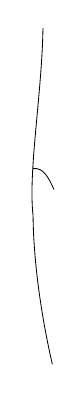
\begin{tikzpicture}[x=.7cm,y=.7cm]
\draw[line width=.3pt] (.42,6.1) .. controls (.40,4.9) and (.15,3.5) .. (.24,2.7) .. controls (.25,1.7) and (.44,.65) .. (.59,0);
\draw[line width=.3pt] (.24,3.55) .. controls (.43,3.58) and (.53,3.37) .. (.62,3.17);
\end{tikzpicture}}}

\uline{Corollaire à la demonstration du lemme $\underline{\overline{\mathrm{VIII}}}$.} \margin{!!}

Si $\Gamma$ est un polygone il existe un couple de sommets \inserted{distincts}\margin{\figure{\begin{tikzpicture}[x=.5cm,y=.5cm]
\draw[line width=.3pt] (-.15,-.95) .. controls (-.35,-.25) and (.10,-.25) .. (1.05,-.20) .. controls (2.1,-.16) and (2.95,.00) .. (3.18,.35);
\end{tikzpicture}}} $s,s'\in S(\Gamma)$ tels que $s'$ est \deleted{\unsure{vis}} $(\mathbb{R}^2-\Gamma)$-visible de $s$ et $]s',s[\subset\partial E(\Gamma)$.
% archive sheet number: 36
